%Notes by Harsh Mistry 
%CS 350
%Based on Template From  https://www.cs.cmu.edu/~ggordon/10725-F12/template.tex

\documentclass[twoside]{article}
\setlength{\oddsidemargin}{0.25 in}
\setlength{\evensidemargin}{-0.25 in}
\setlength{\topmargin}{-0.6 in}
\setlength{\textwidth}{6.5 in}
\setlength{\textheight}{8.5 in}
\setlength{\headsep}{0.75 in}
\setlength{\parindent}{0 in}
\setlength{\parskip}{0.1 in}
\usepackage{amsmath,amsfonts,graphicx}
\newcounter{lecnum}
\renewcommand{\thepage}{\thelecnum-\arabic{page}}
\renewcommand{\thesection}{\thelecnum.\arabic{section}}
\renewcommand{\theequation}{\thelecnum.\arabic{equation}}
\renewcommand{\thefigure}{\thelecnum.\arabic{figure}}
\renewcommand{\thetable}{\thelecnum.\arabic{table}}
\newcommand{\lecture}[4]{
   \pagestyle{myheadings}
   \thispagestyle{plain}
   \newpage
   \setcounter{lecnum}{#1}
   \setcounter{page}{1}
   
   \graphicspath{ {images/} }
   
%Info Box 
   \begin{center}
   \framebox{
      \vbox{\vspace{2mm}
    \hbox to 6.28in { {\bf CS 458/658 - Computer Security and Privacy
	\hfill Fall 2018} }
       \vspace{4mm}
       \hbox to 6.28in { {\Large \hfill Lecture #1: #2  \hfill} }
       \vspace{2mm}
       \hbox to 6.28in { {\it Lecturer: #3 \hfill Notes By: #4} }
      \vspace{2mm}}
   }
   \end{center}
   
   \markboth{Lecture #1: #2}{Lecture #1: #2}



 
}

\renewcommand{\cite}[1]{[#1]}
\def\beginrefs{\begin{list}%
        {[\arabic{equation}]}{\usecounter{equation}
         \setlength{\leftmargin}{2.0truecm}\setlength{\labelsep}{0.4truecm}%
         \setlength{\labelwidth}{1.6truecm}}}
\def\endrefs{\end{list}}
\def\bibentry#1{\item[\hbox{[#1]}]}

\newcommand{\fig}[3]{
			\vspace{#2}
			\begin{center}
			Figure \thelecnum.#1:~#3
			\end{center}
	}

\newtheorem{theorem}{Theorem}[lecnum]
\newtheorem{lemma}[theorem]{Lemma}
\newtheorem{ex}[theorem]{Example}
\newtheorem{proposition}[theorem]{Proposition}
\newtheorem{claim}[theorem]{Claim}
\newtheorem{corollary}[theorem]{Corollary}
\newtheorem{definition}[theorem]{Definition}
\newenvironment{proof}{{\bf Proof:}}{\hfill\rule{2mm}{2mm}}
\newcommand\E{\mathbb{E}}


%Start of Document 
\begin{document}

\lecture{2}{September 11, 2018}{Ian Goldberg }{Harsh Mistry}

\section{Program Security}

\begin{itemize}
\item writing secure programs is difficult because of Murphy's law and the fact that security relevant programs will always have security bugs
\end{itemize}

\subsection{Flaws, Faults, and Failures}
\begin{itemize}
\item A flaw is a problem
\item There are typically two types of flaws. 
\begin{itemize}
\item \textbf{Faults} - A potential problem (Inside view), so a potential  issue in the code. 
\item \textbf{Failures} - A failure is when something actually goes wrong (outside view)
\end{itemize}
\item Every failure is the result of a flaw, but not every flaw yields a failure. 
\end{itemize}

\subsubsection{Methods for finding flaws}
\begin{itemize}
\item \textbf{Root Cause Analysis } : You can work backwards from a failure 
\item \textbf{Penetrate and Patch} : \textit{Think like an attacker} and intentionally cause failures, then issue a patch
\end{itemize}

\subsubsection{Problems with patching}
\begin{itemize}
\item When patching, pressure is typically high which can cause focus to be narrowed onto a specific failure. This may prevent the programmer from thinking of broader issues.
\item The patched  fault may have caused other failures, which may not be known
\item The patch may introduce new faults
\end{itemize}

\subsubsection{Developing to the specification }
Adding additional behaviour can have security consequences and lead to unexpected behaviour. Given this, when implementing a security/privacy application, the spec must be complete. The application must also match the specification exactly. There should be no additional features. Looking at code is typical the best way to ensure there is no additional exploits and to ensure the spec is met with a high degree of accuracy. 

\subsection{Security flaw types}
\begin{itemize}
\item Unintentional : Most flaws are unintentional
\item Intentional 
\begin{itemize}
\item Malicious
\begin{itemize}
\item General 
\item Targeted 
\end{itemize}
\item Non-Malicious 
\end{itemize} 
\end{itemize}

\subsection{Unintentional Flaws}

Unintentional flaws are the most common type of flaw and occur when the developers mental model does not match the real model. 
Types of unintentional flaws are 
\begin{itemize}
\item Buffer Overflows
\item Integer Overflows
\item Format String Vulnerabilities
\item Incomplete Mediation  
\item TOCTTOU Errors
\end{itemize}

\subsubsection{Buffer Overflows}
\begin{itemize}
\item Buffer overflow is when a large amount of data is written into a location which  is smaller than the data to copy/write.  This causes memory outside the data location to be overridden
\item If programs can write data to indices outside the desired location, an attacker can modify things like saved return addresses, which could cause the program to jump elsewhere on return
\begin{center}
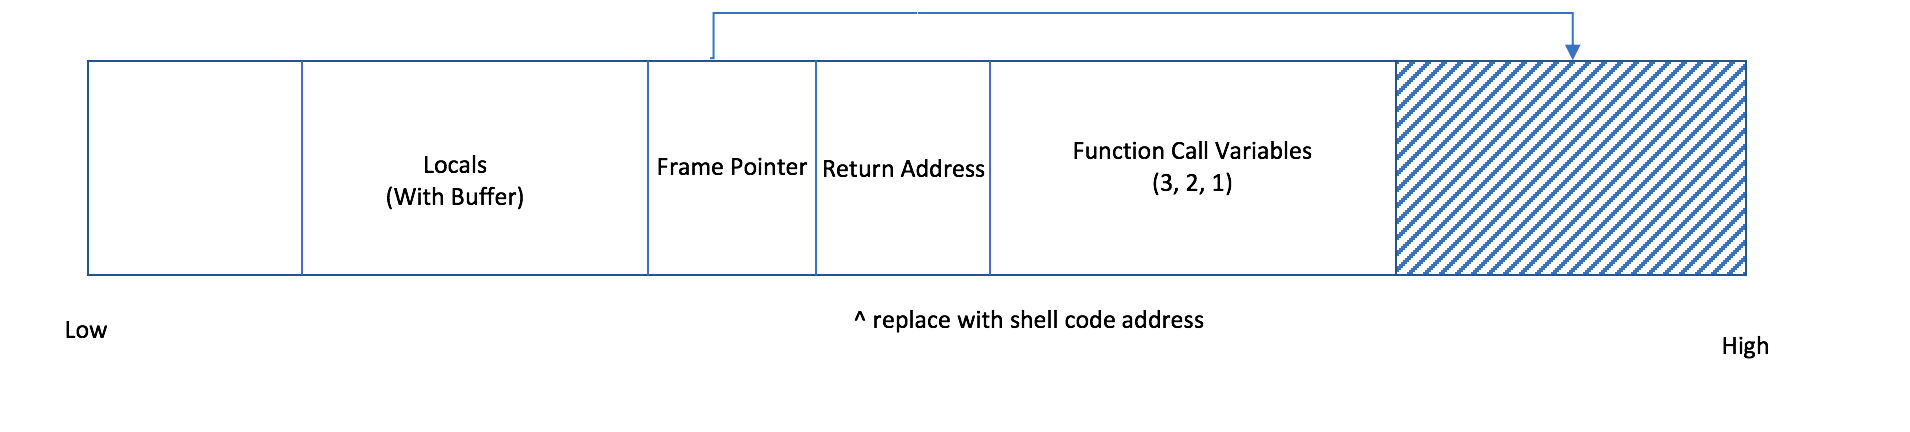
\includegraphics[scale=0.5]{1}
\end{center}
\item Defences
\begin{itemize}
\item Use language with bound checking
\item Computer can put padding between data and return addresses and check if stack data has been overwritten
\item Hardware can provide ability for non-executable stack, so no code  on the stack can be run.
\item OS can place parts of stack at random virtual addresses 
\end{itemize}
\end{itemize}

\subsubsection{Integer Overflow}
\begin{itemize}
\item Integer overflow/underflow is when a machine integer wraps around due to the system system reaching the maximum/minimum values the architecture can handle. 
\item A attacker can exploit this by passing values to a program that will trigger overflow. 
\end{itemize}

\subsubsection{Format String Vulnerabilities}
\begin{itemize}
\item If \verb|printf(buffer)| is used instead of \verb|printf("%s", buffer)|, an attacker can replace the printed valued with their own format string to cause unexpected behaviour or arbitrary code execution 
\item \verb|"%s%s%s"| could cause a crash, \verb|"%x%x%x%x"| could dump parts of the stack, and \verb|%n| can write an address to the stack
\end{itemize}

\subsubsection{Incomplete mediation  }
\begin{itemize}
\item Incomplete mediation occurs when the application accepts incorrect data from the user
\item Incomplete mediation could also lead to SQL injection or buffer overflows. 
\end{itemize}

\end{document}





